!en \section{Let there be light!}
!de \section{Es werde Licht!}

!en The first sample in this chapter is the smallest program I can think of which does something.

!de Das erste Beispiel in diesem Kapitel ist das kleinste Programm, das ich mir vorstellen kann, das tatsächlich auch etwas sichtbares tut.



!en This program will switch on the LED on your Arduino pin 13.

!de Es schaltet die LED am Arduinoanschluss 13 ein.



!en Programming in Assembler means you're in control. But as you know, power requires knowledge and responsibility. If you're entering the world of assembly programming, you have absolute power if you wish to or not. Consequently you need knowledge to become responsible.

!de In Assembler Programmieren heisst, Du hast die Macht! Aber wie wir wissen, erfordert Macht Wissen und Verantwortungsbewusstsein. Jemand der Micro Controller in Assembler programmiert, hat die absolute Macht, ob er es will oder nicht! Demzufolge ist ein Mindestmass an Fachwissen erforderlich um verantwortlich zu handeln.



!en At first you need to know what 'Arduino pin 13' really means. As consequence of the Arduino design it is not pin 13 on your \at. Knowing this is yet the half way thru. Knowing the pin is a step you need to know if are working with a plain chip. What you need to know is the micro controllers internal addressing for Arduino pin 13. To find out, look at \url{http://www.arduino.cc/hu/Hacking/PinMapping}.

!de Als erstes musste Du wissen, was Anschluss 13 am Arduino in Wirklichkeit heisst. Infolge des Arduinodesigns ist Anschluss 13 am Arduino nicht Pin 13 am \at. Das zu wissen ist erst die halbe Miete. Das tatsächliche Pin am \at zu kennen ist erforderlich um mit dem blanken Chip zu arbeiten. Was Du ausserdem wissen musst ist, wie dieser Anschluss im Micro Controller adressiert werden muss. Um das alles heraus zu finden gibt es ein sehr schönes Schaubild: \url{http://www.arduino.cc/hu/Hacking/PinMapping}


\begin{figure}[htbp]
  \centering
  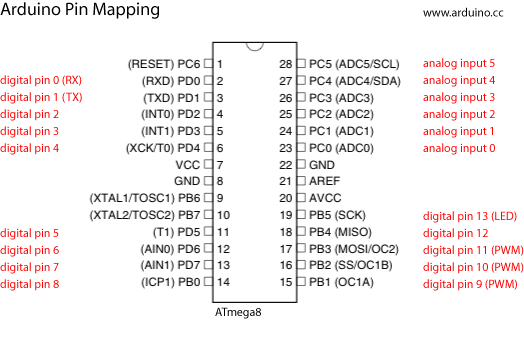
\includegraphics[width=120mm]{Media/www-arduino-cc_Arduino-To-Atmega8-Pins.png}
  \caption{Arduino to \at pins}
  \label{arduino-to-atmega-pins}
\end{figure}

!en After we know everything we need to know to be responsible, we generate our 8byte program that will set our 'LED 13' under power.

!de Nachdem wir zunächst vermutlich genug wissen um verantwortungsvoll zu handeln, programmieren wir unser 8 Byte grosses Programm , dass 'Adruino LED 13' erleuchtet.


\begin{lstlisting}
; LED/S000_let-there-be-light.asm

.DEVICE atmega8

.org 0x0000
            rjmp    start 

start:
            sbi     DDRB,         5
            sbi     PORTB,        5
            
main:
            rjmp    main
\end{lstlisting}

!en As simple as the program is, I believe there is some need for explanation.

!de So einfach dieses Programm auch ist, es gibt doch ein paar Kleinigkeiten zu beleuchten.

At first we have to declare the type of micro controller we are intended to use with the program. This is necessary because different micro controllers do have different assignments in their inner structure and need different addressing for their components. We do this by:

\begin{lstlisting}
.DEVICE atmega8
\end{lstlisting}

Next we need to declare where our world will begin. Funny thing is, we will never really know! So we are forced to use symbols to deal with this necessity. As indicated below, different micro controllers will have different inner values. But not only this, to be honest, where our program lives is due to additional effects a most uncertain thing. We come to this later in the book.

As we are forced to use symbols, we have to do so. We will set a symbol to our programs starting point later and this symbol will be named 'start' in out code. Whatever starts our program it must be informed where to goto to do so:

\begin{lstlisting}
.org 0x0000
            rjmp     start 
\end{lstlisting}

With '.org' (don't forget the leading dot!) we build a sequence of command positioned at the addressed position. This sequence, some times named a table, is a list of actions to do for different requests. At the moment he only request we have is to start our program and fortunately the entry for this request is expected as the first in our table.

For those who really want to know: The addressing in this table is relative to wherever it is placed in real life! So it always starts with 0. Strictly speaking, at this point we already enter the realms of a dreamworld. We don't know what really happens! But sometimes we don't need to. To declare our first magic point, we only need to postulate:

\begin{lstlisting}
start:
\end{lstlisting}

'start:'  is a label and represent the final address for the first memory position used afterwards. In our case the address of the first command in our program.

The next label is already behind all things we need to do in our program. It is the starting point of an unconditional infinite loop. This sequence is necessary because the processor (CPU) of our micro controller (MC) is running as long as it has power. We can't stop it, so we have to lead it into a controlled way of doing 'nothing' because we don't wish our MC to do anything after it did all things we expected it to do.

Between 'start:' und 'main:' is our program. I call this the 'first form of a standard program'. A program which runs ones after the system awakes. Such program may be of limited use, but not completely useless. And the schema of this 'first form' is the basic schema of all derived form. The program 

\begin{itemize}
  \item  starts
  \item  does something
  \item  loops forever, possibly doing something
\end{itemize}

If the program does something inside the 'infinite loop' then this may be called the 'second form of a standard program'. A third form should be expected to pop into existence later on. But anyway. Our program of the first form is specifically designed to show some important rules for good programming.

The two commands which full fill our programs mission will do two things:

\begin{itemize}
  \item  declare pin 5 at PORTB as output pin
  \item  set pin 5 at PORTB under power to enlighten our LED
\end{itemize}

\begin{lstlisting}
            sbi     DDRB,         5
            sbi     PORTB,        5
\end{lstlisting}

Finally the never ending loop:

\begin{lstlisting}
main:
            rjmp    main
\end{lstlisting}

This is all the program does and there is nothing more about it. You will discover, that this program demonstrates prudence and thrift. 

A PORT of an 8bit MC controls eight bit unsung eight pins on the outside. In our \at each one of these pins can be used to:

\begin{itemize}
  \item Put a signal to his pin
  \item Read a signal from its pin which may be +5V or GND as 1 or 0
  \item Read a signal from its pin which may be 'not GND' oder GND as 1 or 0
\end{itemize}

Each pin as can be controlled to do one of these things freely, independent of all the other pins on the same port.

On some pins are additional features possible like

\begin{itemize}
  \item power saving modes
  \item PWM modes
  \item analog to digital converting
  \item interrupts
\end{itemize}

In our program we use the command \texttt{sbi} to set pin 5 instead of the alternative command \texttt{out} with parameter \texttt{1 << 5} which would do the same but not really the same. We wish to manipulate pin 5 only! \texttt{out} would not only send 1 to pin 5 but also 0 to all other pins.

Even if we - at the moment - know that all other pins are unused, we face to situations:

\begin{enumerate}
  \item We will become less and less sure about the usage of pins we don't use in a particular situation.
  \item We don't know what happens if we send 0's to pins we don't know.
\end{enumerate}

\emph{One major concept of good programming is, to do as less as any possible.}

If there is nothing to be done, don't do it! Especially in micro controllers where action means energy loss! So if we need to manipulate a bit, we should not manipulate others bits except we have a good reason to do so. Currently we have not.

We don't want to wake up pins if they could sleep in peace. Because possibly, these otherwise unused pins will eat up our energy.

